\documentclass[UTF8]{ctexart} %使用ctex包,中文支持
\usepackage{amsmath}  %数学公式
\usepackage{graphicx} %插图
\usepackage{fancyhdr} %个性化页眉页脚
\usepackage{geometry} %页边距
\usepackage{bm}  % 公式加粗
\usepackage{float} %为了在分栏下插入图片
\usepackage{ulem}  % 换行下划线
%\usepackage{setspace} %行间距 
\usepackage{ulem} %删除线
\usepackage{multicol} %用于实现在同一页中实现不同的分栏
\geometry{a4paper,left=2cm,right=2cm,top=2cm,bottom=2cm} % 页边距设置

\title{概率图模型笔记}
\author{宋佳欢}
\pagestyle{plain}

\begin{document}
	\maketitle
	\tableofcontents
	\songti \zihao{-4}
	
	
	\section{绪论}
		概率图的三个方面:
		
		1.表示:有向图(贝叶斯网络),无向图(马尔科夫网络),高斯图
		
		2.推断:精确推断,近似推断:确定性近似(变分推断),随机近似:MCMC
		
		3.学习:参数学习,图结构学习
		
		\subsection{基础概念}
			高维随机变量的概率:\[P(x_1,x_2,...,x_p)\]
			
			边缘概率:\[P(x_i)\]
			
			条件概率:\[P(x_j|x_i)\]
		
			加法法则(计算边缘概率):\[P(x_i) = \int P(x_1,x_2)dx_2\]
			
			乘法法则(计算联合概率):\[P(x_1,x_2) = P(x_1)\cdot P(x_2|x_1)\]
			
			链式法则(乘法的推广):\[P(x_1,x_2,\cdots,x_p) = \prod_{i=1}^pP(x_i|x_1,x_2,\cdots,x_{i-1},x_{i+1},\cdots, x_p)\]
			
			贝叶斯定理:
			\[P(x_2|x_1)=\frac{P(x_1,x_2)}{P(x_1)} = \frac{P(x_1,x_2)}{\int P(x_1,x_2)dx_2} = \frac{P(x_2) P(x_1|x_2)}{\int P(x_2) P(x_1|x_2)dx_2}\]
			
		\subsection{条件独立性}	
			\textbf{困境:}$P(x_1,x_2,...,x_p)$计算复杂,所以要简化:
			
			1.假设各个变量之间相互独立(朴素贝叶斯):$P(x|y) = \prod_{i=1}^pP(x_i|y)$
			
			2.现实性每个变量之间多少是有关联的,所以条件再放松一点,那就是马尔可夫性,\[x_j\perp x_{i+1}|x_i,\quad j<i\]
			                                                                         
			3.再推广,\textbf{条件独立性} 假设:f
			\[x_A\perp x_B|x_C,\quad x_A,x_B,x_C\text{是集合,且不相交}\]
			
			条件独立性使用图来表示,在图上赋予概率的意义,使得图能表达条件独立性。
	
	\section{指数族分布}
		\begin{figure}[H]
			\centering{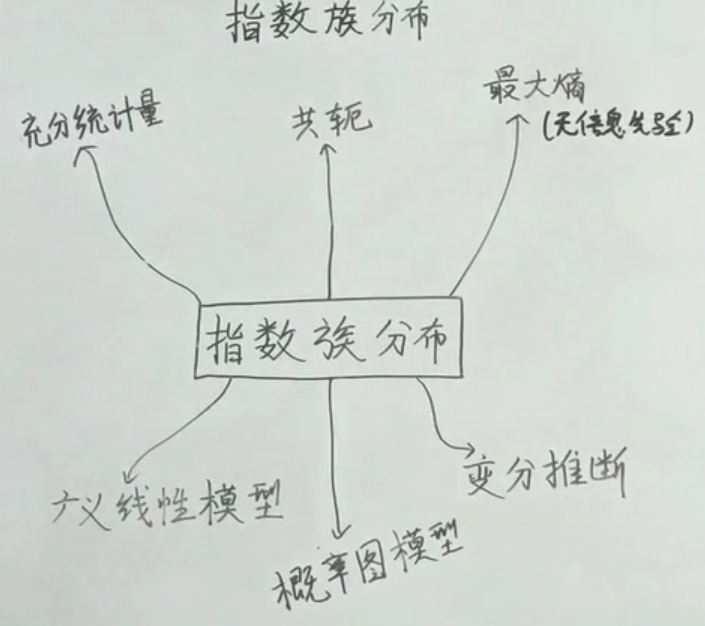
\includegraphics[scale=0.4]{9.png}}
		\end{figure}
		指数族分布的形式:
		\[P(x|\eta) = h(x)exp(\eta^T\varphi(x)-A(\eta))\]
		
		其中$\eta$为参数向量。$\varphi(x)$为充分统计量(给了充分统计量就能描述分布了)。
		$A(\eta)$:log partition function(对数配分函数)。相当与归一化因子,如:
		\[P(x|\theta) = \frac{1}{Z}\hat{P}(x|\theta)\]
		\[\text{两边对x积分,化简得到:}Z = \int \hat{P}(x|\theta)dx \]
		
		\subsection{高斯分布指数族形式}
			\[P(X|\theta) = \frac{1}{\sqrt{2\pi }\sigma}exp\big(-\frac{(x-\mu)^2}{2\sigma^2}\big)\]
			将x与参数分开:
			\[
			\begin{aligned}
			P(X|\theta) &= \frac{1}{\sqrt{2\pi\sigma^2 }}exp\big(-\frac{1}{2\sigma^2}(x^2-2\mu x+\mu^2)\big)\\
			&= exp[log(2\pi\sigma^2)^{-\frac{1}{2}}]exp\{-\frac{1}{2\sigma^2}(x^2-2\mu x)-\frac{\mu^2}{2\sigma^2}\}\\
			& = exp\{ \underbrace{(\frac{\mu}{\sigma^2} - \frac{1}{2\sigma^2})}_{\eta^T} 
			\underbrace{\begin{pmatrix}	x\\x^2\end{pmatrix}}_{\varphi(x)}
			\underbrace{-(\frac{\mu}{2\sigma^2}+\frac{1}{2}log2\pi\sigma^2)}_{A(\eta)}\}
			\end{aligned}\]
			
			\[\eta = \begin{pmatrix}
			\eta_1\\
			\eta_2
			\end{pmatrix}
			= 
			\begin{pmatrix}
				\frac{\mu}{\sigma^2}\\-\frac{1}{2\sigma^2}
			\end{pmatrix}\]
			\[A(\eta)=-\frac{\eta_1^2}{4\eta_2} + \frac{1}{2}log(-\frac{\pi}{\eta_2})\]
			
		\subsection{对数分配函数与充分统计量之间的关系}
			即$\varphi(x)$与$A(\eta)$之间的关系。
			\[\begin{aligned}
			P(x|\eta) &= h(x)exp(\eta^T\varphi(x)-A(\eta))\\
			&=\frac{1}{exp(A(\eta))}h(x)exp(\eta^T\varphi(x))
			\end{aligned}\]
			利用概率密度函数积分为1的性质,两边积分化简后得到:
			\[exp(A(\eta)) = \int h(x)exp(\eta^T\varphi(x))dx\]
			关于$\eta$求导:
			\[exp(A(\eta))A'(\eta) = \frac{\partial}{\partial\eta}\Big( \int h(x)exp(\eta^T\varphi(x))dx\Big)\]
			\[exp(A(\eta))A'(\eta) = \int h(x)exp(\eta^T\varphi(x))\cdot\varphi(x)dx\]
			\[A'(\eta) = \frac{\int h(x)exp(\eta^T\varphi(x))\cdot\varphi(x)dx}{exp(A(\eta))}\]
			\[A'(\eta) =\int \underbrace{h(x)exp\Big(\eta^T\varphi(x)-A(\eta)\Big)}_{P(x|\eta)}\cdot\varphi(x)dx\]
			\[A'(\eta) =\int P(x|\eta)\cdot\varphi(x)dx = E_{P(x|\eta)}\Big[\varphi(x)\Big]\]
			
			可证$A(\eta)$的二阶导可得为$\varphi(x)$的方差(这里没有证),所以有:
			\[A'(\eta)=E_{P(x|\eta)}\Big[\varphi(x)\Big]\]
			\[A''(\eta)=Var\Big[\varphi(x)\Big]\]
			因为方差为正数,所以$A(\eta)$是凸函数。
		\subsection{极大似然估计与充分统计量}
			 上述讨论并没有引入数据,是根据公式推导的性质。
			 下面对参数$\eta$进行极大似然估计,假设有样本集$D={x_1,x_2,\cdots, x_N}$,则:
			 \[\begin{aligned}
			\eta_{MLE} &= argmaxlogP(D|\eta)\\
			&= argmaxlog\prod_{i=1}^NP(x_i|\eta)\\
			&= argmax\sum_{i=1}^NlogP(x_i|\eta)\\
			&= argmax\sum_{i=1}^Nlog\Big[h(x)exp(\eta^T\varphi(x)-A(\eta))\Big]\\
			&= argmax\sum_{i=1}^N\Big(\eta^T\varphi(x)-A(\eta)\Big)\quad(\text{去除无关的变量})
			 \end{aligned}\]
		
			将上式关于$\eta$求导并置为0:
			\[\begin{aligned}
			\frac{\partial}{\partial\eta}\sum_{i=1}^N\Big(\eta^T\varphi(x)-A(\eta)\Big)&=\sum_{i=1}^N\frac{\partial}{\partial\eta}\Big(\eta^T\varphi(x)-A(\eta)\Big)\\
			&=\sum_{i=1}^N\Big(\varphi(x_i)-A'(\eta)\Big)\\
			&= \sum_{i=1}^N\varphi(x_i)-NA'(\eta)\\
			&=0
			\end{aligned}\]
			得到:
			\[A'(\eta) = \frac{1}{N}\sum_{i=1}^N\varphi(x_i)\]
			求参数$\eta$,再加一步,求A的导数的反函数:
			\[\eta = A'^{(-1)}(\eta)\]
			
			可以得到结论:可以仅保留充分统计量求出参数,样本就可以扔了。
			
		\subsection{最大熵角度}
			在满足已知事实条件下(约束),最大熵的分布就是我们要的分布。若没有任何已知的情况下,均匀分布的熵最大。
			
			\textbf{经验分布}:对已知样本的描述。
			
			有样本$D={x_1,x_2,\cdots, x_N}$,则经验分布:
			
			\[\hat{P}(X=x)=\frac{count(x)}{N}\]
			\[E_{\hat{p}}[x],\quad Var_{\hat{p}}[x]\]
			
			设$f(x)$是任意关于x的函数,已知事实就描述为:
			\[E_{\hat{p}}[f(x)] = \Delta\]
			
			\textbf{最大熵原理:}
			\[min\quad\sum_{x}p(x)logp(x)\]
			\[s.t.\sum_xp(x)=1,\quad E_{p}[f(x)]=E_{\hat{p}}[f(x)]=\Delta\]
			
			我们将$f(x)$推广到多维情形:
			\[f(x)=\begin{pmatrix}
			f_1\\f_2\\\vdots\\f_Q
			\end{pmatrix},
			\Delta =\begin{pmatrix}
			\Delta_1\\\Delta_2\\\vdots\\\Delta_Q
			\end{pmatrix}  \]
			
			利用拉格朗日乘子法求解最大熵模型:
			\[L(p,\lambda_0,\lambda) = \sum_{i=1}^Np(x_i)logp(x_i)+\lambda_0\Big(1-\sum_{i=1}^Np(x_i)\Big)+\lambda\Big(\Delta-E_{p}[f(x)]\Big)\]\
			求偏导置为0:
			\[\frac{\partial L}{\partial p(x_i)} = logp(x_i)+1-\lambda_0-\lambda^Tf(x_i)=0\]
			
			\[logp(x) = \lambda^Tf(x)+\lambda_0-1\]
			\[p(x) = exp\{\underbrace{\lambda^Tf(x)}_{\eta^T\varphi(x)}-\underbrace{(\lambda_0+1)}_{A(\eta)}\]
			
			结论:由最大熵原理推出来的模型就是指数族分布。
		\subsection{共轭分布}
			共轭分布的概念:
				
			当某个分布的先验分布碰上了某种似然函数,其后验分布就会和先验分布的类型相同:
			\[\underbrace{P(\beta|X)}_{\text{后验分布}} \propto \underbrace{P(X|\beta)}_{\text{似然函数}}\underbrace{ P(\beta)}_{\text{先验分布}}\]
			
			当先验与似然都为指数族分布(假设了似然函数为一维):
			\[\begin{aligned}
			P(\beta|X) &\propto \underbrace{h(X)exp\{\beta\varphi(X) - A_l(\beta)\}}_{P(X|\beta)} \cdot \underbrace{h(\beta)exp\{\alpha^T\varphi(\beta) - A(\alpha)\}}_{P(\beta)}\\
			\end{aligned}
			\]
			其中$h(X)$和$A(\alpha)$对于$\beta$来说是常数,下面可以忽略。我们下面做这样的假设:
			\[\varphi(\beta) = \begin{pmatrix}
			\beta\\
			-A_l(\beta)
			\end{pmatrix}\quad
			\alpha = \begin{pmatrix}
			\alpha_1\\
			\alpha_2
			\end{pmatrix}\]
			
			我们得到:
			\[\begin{aligned}
			P(\beta|X) &\propto h(\beta)  exp\{\beta\varphi(X) - A_l(\beta) +\alpha_1\beta -\alpha_2A_l(\beta)  \}\\
			&=h(\beta) exp\{(\varphi(X)+\alpha_1)\beta - ((1+\alpha_1)A_l(\beta))\}\\
			&=h(\beta) exp\{\underbrace{(\hat{\alpha_1},\hat{\alpha_2})}_{\text{新的参数}}\begin{pmatrix}
			\beta\\
			-A_l(\beta)
			\end{pmatrix}\}
			\end{aligned}
			\]
			
			如果似然函数的对数配分函数与先验分布的充分统计量的第二部分相同,那么先验与后验属于同一分布(共轭)。所以指数族分布的似然函数必定能找到一个使得后验分布共轭的先验分布。
			
			
			
		
		
		

	
			
	\section{贝叶斯网络}
		\subsection{贝叶斯网络的三种结构的独立性}
			1.tail to tail
			\begin{figure}[H]
				\centering{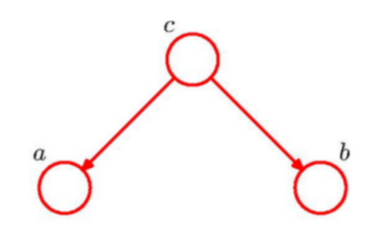
\includegraphics[scale=0.5]{2.png}}
			\end{figure}
			计算三个变量的联合概率:
			\[\text{因子分解:\quad}P(a,b,c) = P(c)P(a|c)P(b|c)\]
			\[\text{链式法则:\quad}P(a,b,c) = P(c)P(a|c)P(b|a,c)\]
			
			可得:\[P(b|c) = P(b|a,c)\Longrightarrow a\perp b|c\]
			
			该图的条件独立性:\textbf{若c被观测,则路径阻塞}(图论的说法,阻塞意味着独立)\\
			
			2.head to tail
			\begin{figure}[H]f
				\centering{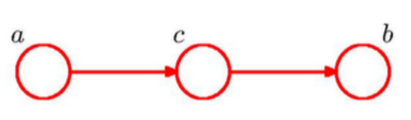
\includegraphics[scale=0.5]{3.png}}
			\end{figure}
			\textbf{若c被观测,则路径阻塞},$a\perp b|c$\\
				
			3.head to head
			\begin{figure}[H]
				\centering{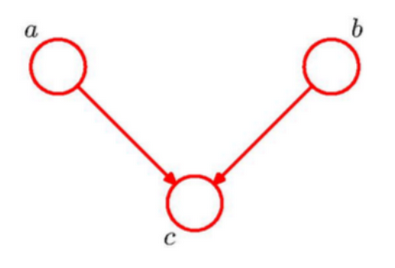
\includegraphics[scale=0.5]{4.png}}
			\end{figure}
			\textbf{若c被观测,则路径是通的,即a,b之间不独立}
			
			一个例子:
			\begin{figure}[H]
				\centering{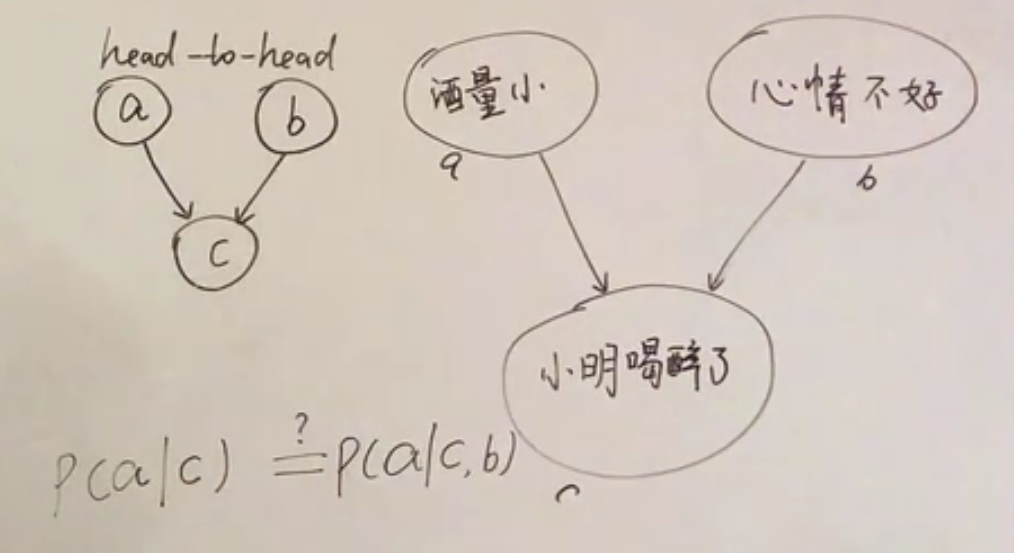
\includegraphics[scale=0.35]{5.png}}
			\end{figure}
			得知小明喝醉,推小明酒量小的概率$P(a|c)$应该是比较大的。
			
			得知小明喝醉且心情不好,推小明酒量小的概率$P(a|c,b)$就比上一种情况小了。因此a,b是相关的。
			
		\subsection{D划分(d-Separation)}
			1.集合A,B,C,通过tail to tail和head to tail结构连接,A到B的路径上的节点都\uline{必须}在C的内部。
			
			2.集合A,B,C,通过head to head结构连接,A到B的路径上的节点以及其后继节点都\uline{不能}在C的内部。
			
			满足上述两个要求,则$A\perp B|C$。即满足全局马尔可夫性。
			
			以下图为例,计算边缘概率$P(x_i|x_1,x_2,\cdots,x_{i-1},x_{i+1},\cdots, x_p)$:
			\begin{figure}[H]
				\centering{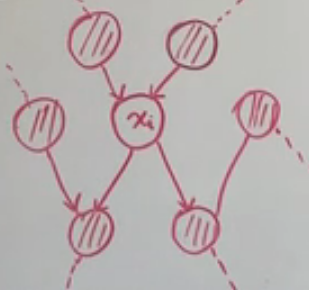
\includegraphics[scale=0.4]{6.png}}
			\end{figure}
			\[\begin{aligned}
			P(x_i|x_1,x_2,\cdots,x_{i-1},x_{i+1},\cdots, x_p) &= \frac{P(X)}{P(x_1,x_2,\cdots,x_{i-1},x_{i+1},\cdots, x_p)}\\
			&=\frac{P(X)}{\int P(X)dx_i}\\
			&=\frac{\prod_{j=1}^pP(x_j|x_{parent(j)})}{\int \prod_{j=1}^pP(x_j|x_{parent(j)})dx_i}\\
			&x_{parent(j)}\text{表示}x_i\text{的父节点们}
			\end{aligned}\]			
			
			可见$x_i$的边缘概率只与和它相关的一些节点有关,即上图中的打阴影的节点,$x_i$周围的一圈又叫马尔可夫毯。
			
			
	\section{Markov网络}	
		全局马尔可夫性:从节点集A中的节点到B中的节点的路径,都经过节点集C中的节点,则$A\perp B|C$。
		
		局部马尔可夫性:$a\perp \{\text{全集}-a-\text{邻居}\}|\text{邻居}$。
		
		成对马尔可夫性:$x_i\perp x_j|\{\text{全集}-x_i-x_j\}$ 
		
		团:图中节点的一个子集,其中任意两个节点有互相连接。
		
		极大团:在极大团中再加入一个节点就不够成团。
		
		因子分解(极大团的势函数相乘):
		\[P(X) = \frac{1}{Z}\prod_{i=1}^k \psi(x_{C_i})\]
		
		
		
	\section{推断inference}
			\textbf{目的:}
			
			求联合概率: $P(x_1,x_2,...,x_p)$
			
			求边缘概率:$P(x_i) = \sum_{x_1}\cdots\sum_{x_{i-1}}\sum_{x_{i+1}}\cdots\sum_{x_p}P(X)$
			
			求条件概率:$P(x_A|x_B)$
			
			最大化后验概率: $\hat{Z}=arg\max_{Z}P(Z|X) \propto argmaxP(Z,X)$
			
			\textbf{精确推断:}
			
			变量消去(variable elimanation) ,信念传播(belief propagation)(Sum-product 针对树结构),junction tree(普通图结构)。
			
			\textbf{近似推断:}
			
			loop belief propagation(有环图), import sampling, MCMC, Variational Inference。
		\subsection{变量消去(variable elimanation)}
			以马尔可夫链为例:
			\[\textcircled{a}\rightarrow\textcircled{b}\rightarrow\textcircled{c}\rightarrow\textcircled{d}\]
			\[P(d) = \sum_{a,b,c}P(a,b,c,d) = \sum_{a,b,c}P(a)P(b|a)P(c|b)P(d|c)\]
			用上面的公式直接计算边缘概率,计算量会随着可选状态数增加而指数增加,因此需要化简。可以看到,关于a求和时,求和符号内的有些项式与a无关的,可以提出去,可以写成:
			\[\begin{aligned}
			P(d) &=  \sum_{a,b,c}P(a)P(b|a)P(c|b)P(d|c)\\
			&= \sum_{b,c}P(c|b)P(d|c)\underbrace{\sum_aP(a)P(b|a)}_{\varphi_a(b)}\\
			&= \sum_cP(d|c)\underbrace{\sum_bP(c|b)\varphi_a(b)}_{\varphi_b(c)}\\
			&= \varphi_c(d)
			\end{aligned}\]
			
			(乘法分配率)
			
		\subsection{信念传播(belief propagation)}
			如下图所示,如果计算无向图中节点a的概率:
			\[P(a) = \sum_{b,c,d}P(a,b,c,d)\]
			\[P(a,b,c,d) = \frac{1}{Z}\varphi_a(a)\varphi_b(b)\varphi_c(c)\varphi_d(d)\varphi_{a,b}(a,b)\varphi_{b,c}(b,c)\varphi_{b,d}(b,d),\quad\text{(四个点,三条边)}\]
			\begin{figure}[H]
				\centering{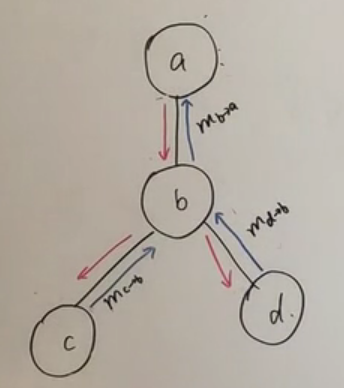
\includegraphics[scale=0.5]{8.png}}
			\end{figure}
			
			可以先计算与c或d相关的项:
			\[m_{c\rightarrow b}(b) =\sum_c\varphi_c(c) \varphi_{b,c}(b,c)\]
			\[m_{d\rightarrow b}(b) =\sum_d\varphi_d(d) \varphi_{b,d}(b,d)\]
			
			再计算$m_{b\rightarrow a}$:
			\[m_{b\rightarrow a}(a) = \sum_b\varphi_b(b)\varphi_{a,b}(a,b)m_{c\rightarrow b}(b)m_{d\rightarrow b}(b)\]
			
			最后得到a的边缘概率:
			\[P(a) = \varphi_a(a)m_{b\rightarrow a}(a)\]
			
			跳出这个例子,得到更加普遍的计算方式:
			\[m_{j\rightarrow i}(x_i) = \sum_{x_j}\varphi_{ij}\underbrace{\varphi_j \prod_{k\subset NB(j)-i}M_{k\rightarrow j}(x_j)}_{belief(i)}\]
			\[P(x_i) = \varphi_i \prod_{k\subset NB(i)}M_{k\rightarrow i}(x_i)\]
			其中$NB(j)-i$表示除了$x_i$以外,$x_j$的所以邻居节点的集合。
			
			还以上图为例,上面公式可以理解成每个节点都在收集关于a的信息,b从c,d中收集关于a的所以信息,然后再送到a。beilef(b)即表示为在b到a这条路径上b所能提供的信息量。
			
			BP算法所做的事情就是遍历整个图,计算所有的$m_{ij}$,然后在到处边缘概率。分为下面几步:
			
			1.选个一个根节点
			
			2.收集信息
			
			3.发送信息
		\subsection{Max-product Algorithm}
			该算法可看成BP的改进,Viterb的推广。
			
			重新定义$m_{j\rightarrow i}$:
			\[m_{j\rightarrow i}(x_i) = \max_{x_j}\varphi_{ij}\varphi_j \prod_{k\subset NB(j)-i}M_{k\rightarrow j}(x_j)\]
			找到一个最优的$\max_{x_j}$的状态,使得$m_{j\rightarrow i}$达到最大。
			\\
		\section{变分推断(Variational Inference)}
			\subsection{引入}
				贝叶斯推断(求后验分布):
				\[\underbrace{P(\theta|X)}_{\text{后验概率}} = \frac{P(X|\theta)P(\theta)}{\underbrace{P(X)}_{\int _\theta P(X|\theta)P(\theta)d\theta}}\]
				
				贝叶斯决策(计算新样本的后验概率):
				假设给定了N个观测数据X,新的样本$\tilde{x}$,求$P(\tilde{x}|X)$:
				
				引入参数$\theta$:
				\[P(\tilde{x}|X) = \int_{\theta}P(\tilde{x},\theta|X)d\theta\]
				\[\begin{aligned}
				P(\tilde{x}|X) &= \int_{\theta}P(\tilde{x}|\theta,X)\underbrace{P(\theta|X)}_{\text{后验}}d\theta\\
				&= \int_{\theta}P(\tilde{x}|\theta)P(\theta|X)d\theta \quad (\text{给定了}\theta,X\text{与}\tilde{x}\text{无关})\\
				&=E_{P(\theta|X)}[P(\tilde{x}|\theta,X)]
				\end{aligned}			
				\]
				
				所以可以用推断求得的后验去预测新的样本。
				
				问题主要集中在求后验分布(推断),如果非常简单,就可以通过精确推断求解,但是常常参数或隐变量的空间维度特别高,很难取求解那个积分,所以可通过近似推断来求解。
			\subsection{推导}
				X: observed data
				
				Z: latent variable + paramter
				
				(X,Z): complete data
				
				\[\begin{aligned}
				lnP(X) &= lnP(X,Z) - lnP(Z|X)\\
				&= ln\Bigg(\frac{P(X,Z)}{q(Z)}\Bigg) - ln\Bigg(\frac{P(Z|X)}{q(Z)}\Bigg)\\
				&=  lnP(X,Z) -lnq(Z) - ln\Bigg(\frac{P(Z|X)}{q(Z)}\Bigg)
				\end{aligned}\]
				两边求关于分布$q(X)$的期望:
				\[lnP(X) = \underbrace{\int_ZlnP(X,Z)q(Z)dZ - \int_Zlnq(Z)q(Z)dZ}_{ELBO}  \underbrace{-\int_Zln\Bigg(\frac{P(Z|X)}{q(Z)}\Bigg)q(Z)dZ}_{KL\text{散度}(\geq0)}\]
				所以$lnP(x)$是ELBO的上界。
				
				从另一角度来推导:
				\[\begin{aligned}
				lnP(X)& = ln\Big(\int_ZP(X,Z)dZ\Big)\\
				&= ln\Big(\int_Z\frac{P(X,Z)}{q(Z)}\cdot q(Z)dZ\Big)\\
				&= lnE_{q(Z)}\Big[\frac{P(X,Z)}{q(Z)}\Big]\\
				&\geq E_{q(Z)}\Big[ln\frac{P(X,Z)}{q(Z)}\Big]\quad (\text{琴生不等式})\\
				& = \underbrace{E_{q(Z)}\Big[lnP(X,Z)\Big] - E_{q(Z)}\Big[lnq(Z)\Big]}_{ELOB}
				\end{aligned}\] 
				
				我们想让分布$q(Z)$与后验分布$P(Z|X)$尽可能相似,当两个分布相同时,KL散度为0,ELBO达到最大与似然函数$lnP(X)$相等。所以目标就找到一个分布$q(Z)$使得ELBO最大化。
				
				选择一个简单的分布q(Z),每一个维度都统计独立:
				\[q(Z) = \prod_{i=1}^Mq_i(Z_i)\]
				
				代入$q(Z)$,ELOB就改写为:
				\[L(q) =\underbrace{\int_Z\prod_{i=1}^Mq_i(Z_i)lnP(X,Z)dZ}_{part_1} - \underbrace{\int_Z\prod_{i=1}^Mq_i(Z_i)\sum_{i=1}^Mlnq_i(Z _i)dZ}_{part_2} \]
				
				先化简part-1:
				\[\begin{aligned}
				part_1 &= \int_{Z_1}\int_{Z_2}\cdots\int_{Z_M}\prod_{i=1}^Mq_i(Z_i)lnP(X,Z)dZ_1dZ_2\cdots dZ_M\\
				&= \int_{Z_j} q_j(Z_j)\Bigg(\int_{i\neq j}\cdots\int\prod_{i\neq j}^Mq_i(Z_i)lnP(X,Z)\prod_{i\neq j}^MdZ_i\Bigg)dZ_j\\
				& =  \int_{Z_j} q_j(Z_j)\Bigg(\int_{i\neq j}\cdots\int lnP(X,Z)\prod_{i\neq j}^Mq_i(Z_i)dZ_i\Bigg)dZ_j\\
				& = \int_{Z_j} q_j(Z_j)\Bigg[E_{\prod_{i\neq j}^Mq(Z_i)}\bigg[lnP(X,Z)\bigg]\Bigg]dZ_j
				\end{aligned}\]
			
				part-2部分:
					\[
					\begin{aligned}
					part_2 &=\int_Z\prod_{i=1}^Mq_i(Z_i)\sum_{i=1}^Mlnq_i(Z _i)dZ\\
					&=\int_Z\prod_{i=1}^Mq_i(Z_i)[logq_1(Z_1)+logq_2(Z_2)+\cdots+logq_M(Z_M)]dZ\\
					& = \underbrace{\int_Z\prod_{i=1}^Mq_i(Z_i)logq_1(Z_1)dZ}_{\text{第一项为例}} +\cdots\\
					& = \int_{Z_1Z_2\cdots Z_M}q_1(Z_1)q_2(Z_2)\cdots q_M(Z_M)logq_1(Z_1)dZ_1dZ_2\cdots dZ_M +\cdots\\
					& = \int_{Z_1}q_1(Z_1)logq_1(Z_1)dZ_1 \cdot \underbrace{\int_{Z_2\cdots Z_M}q_2(Z_2)\cdots q_M(Z_M)dZ_2\cdots dZ_M}_{=1}+\cdots\\
					&= \sum_{i=1}^M\Bigg(\int_{Z_i}q_i(Z_i)lnq(Z_i)dZ_i\Bigg)
					\end{aligned}\]
				推导参考EM的Q函数化简。如果我们只对$Z_j$感兴趣:
				\[part_2 = \int_{Z_j}q_j(Z_j)lnq(Z_j)dZ_j +C\]
				
				所以将化简后的两部分合起来:
				\[L(q_j) = \int_{Z_j} q_j(Z_j)\Bigg[\underbrace{E_{\prod_{i\neq j}^Mq_i(Z_i)}\bigg[lnP(X,Z)\bigg]}_{ln\tilde{p}(X,Z_j)}\Bigg]dZ_j - \int_{Z_j}q_j(Z_j)lnq_j(Z_j)dZ_j +C\]
				\[\begin{aligned}
				L(q_j) &= \int_{Z_j}q_j(Z_j)ln\frac{ln\tilde{p}(X,Z_j)}{lnq_j(Z_j)}dZ_j +C\\
				&=-KL(q_j\|\tilde{p}(X,Z_j))\leq 0
				\end{aligned}\]
			
			\subsection{应用}
			接下来对下标做一下规范,用上标来表示第几个样本,下标表示变量的维度。
			
			\qquad$x$观测样本$\rightarrow X=\{x^{(i)}\}_{i=1}^N$
			
			\qquad$z$隐变量$\rightarrow Z=\{z^{(i)}\}_{i=1}^N$
			
			所以似然函数:
			\[logP_\theta(X) = \sum_{i=1}^NlogP_\theta(x^{(i)})\]
			
			单个样本的似然函数又可写成:
			\[logP_\theta(x^{(i)}) = \underbrace{ELBO}_{L(q)} + \underbrace{KL(q||p)}_{\geq0}\]
			
			最大化数据集的似然函数,就要最大化每个样本的似然函数,目标函数为:
			\[\hat{q} = arg\min_qKL(q||p) = arg\max_qL(q)\]
			
			通过平均场理论,得到假设:
			\[q(z) = \prod_{i=1}^Mq_i(z_i)\]
			其中的$z_i$可认为是最大团的概念。
			
			\textbf{迭代式:}
			\[\begin{aligned}
			logq_j(z_j) &= E_{\prod_{i\neq j} q_i(z_i)}\Big[logP_\theta(x^{(i)},Z)\Big]+C\\
			& = \int_{q_{i\neq j}}q_1q_2\cdots q_{j-1}q_{j+1}\cdots q_{M}\Big[logP_\theta(x^{(i)},Z)\Big]dq_{i\neq j}
			\end{aligned}\]
			比如在求$q_1$时,固定了除$q_1$以外其他参数不动,在求下一个$q_2$时,,用新的$q_1$替换掉旧的,且固定其他参数不动。不断迭代(坐标上升)。但是基于平均场的方法,对很多问题还是无法求解的,因为它的假设太强了。
			
			\subsection{SGVI}
				求后验分布$q(Z|X)$等价求其分布的参数$\phi$,所以更新公式可以改写为:
				\[\hat{\phi} = arg\max_{\phi}\underbrace{L(\phi)}_{ELBO}\]
				
				\[\begin{aligned}
				ELBO & = E_{q_\phi(Z)}\Big[\frac{log\tilde{p}(x^{(i)},Z)}{logq_\phi(Z)}\Big] \\
				& = E_{q_\phi(Z)}\Big[log\tilde{p}(x^{(i)},Z)-logq_\phi(Z)\Big]\\
				&=L(\phi)
				\end{aligned}\]
				
				接下来求$L(\phi)$关于$\phi$的梯度:
				\[\begin{aligned}
				\nabla_\phi L(\phi) &= \nabla_\phi  E_{q_\phi(Z)}\Big[log\tilde{p}(x^{(i)},Z)-logq_\phi(Z)\Big]\\
				&= \nabla_\phi  \int_{q_\phi(Z)}q_\phi(Z)\Big[log\tilde{p}(x^{(i)},Z)-logq_\phi(Z)\Big]dZ\\
				&= \underbrace{\int\nabla_\phi q_\phi(Z)\Big[log\tilde{p}(x^{(i)},Z)-logq_\phi(Z)\Big]dZ}_{part_1}+\underbrace{\int q_\phi(Z)\nabla_\phi\Big[log\tilde{p}(x^{(i)},Z)-logq_\phi(Z)\Big]dZ}_{part_2}
				\end{aligned}\]
				先看第二项:
				\[\begin{aligned}
				part_2& =\int q_\phi(Z)\nabla_\phi\Big[log\tilde{p}(x^{(i)},Z)-logq_\phi(Z)\Big]dZ\\
				&= -\int q_\phi(Z) \nabla_\phi logq_\phi(Z)dZ\\
				&= -\int q_\phi(Z)\frac{1}{q_\phi(Z)}\nabla_\phi q_\phi(Z)dZ\\
				& = -\nabla_\phi\int q_\phi(Z)dZ = -\nabla_\phi 1 = 0
				\end{aligned} \]
				
				所以梯度就剩下第一项:
				\[\begin{aligned}
				\nabla_\phi L(\phi) &=\int_{q_\phi(Z)}\nabla_\phi q_\phi(Z)\Big[log\tilde{p}(x^{(i)},Z)-logq_\phi(Z)\Big]dZ\\
				&=\int_{q_\phi(Z)}q_\phi(Z) \nabla_\phi logq_\phi(Z)\Big[log\tilde{p}(x^{(i)},Z)-logq_\phi(Z)\Big]dZ\\
				& = E_{q_\phi(Z)}\Bigg[\nabla_\phi \underbrace{logq_\phi(Z)}_{\text{不稳定}}\Big[log\tilde{p}(x^{(i)},Z)-logq_\phi(Z)\Big]\Bigg])
				\end{aligned}\]
				
				但是如果MCMC采样到的概率$q_\phi(Z)$特别小,在log函数中,这个值就会非常大,造成我们要求期望的量(梯度)的方差特别大,(本来求梯度就是为了逼近我们要求的分布,现在连梯度都不稳定了)这样就需要更多的样本才能更好地近似。所以就不能直接用MCMC采样。
				
				\textbf{重参数化技巧:}
			\subsection{指数族分布+变分推断}
				变分推断中的ELBO(假设有两部分未知参数):
					\[L(q(Z,\beta)) = E_{q(Z,\beta)}[logP(X,Z,\beta)] - E_{q(Z,\beta)}[logq(Z,\beta)]\]
					
				分别写出两个参数的指数族分布形式的似然函数:
				\[P(\beta|Z,X) = h(\beta)exp\{\eta(Z,X)^T\varphi(\beta)-A_g(\eta(Z,X))\}\]
				\[P(Z|\beta,X) = h(Z)exp\{\eta(\beta,X)^T\varphi(Z)-A_l(\eta(\beta,X))\}\]
				这里将参数向量$\eta$看做是$Z,X$或$\beta,X$的函数。
				我们用两个分布去逼近上面两个似然:
				\[q(\beta|\lambda) = h(\beta)exp\{\lambda^T\varphi(\beta)-A_g(\lambda)\}\]
				\[q(Z|\phi) = h(Z)exp\{\phi^T\varphi(Z)-A_g(\phi)\}\]
				我们不断调整参数$\lambda,\phi$,使得这两个分布与似然函数足够接近。所以,我们可以将ELBO看做是$\lambda,\phi$的函数。
				\[L(\lambda,\phi) = E_{q(Z,\beta)}[logP(X,Z,\beta)] - E_{q(Z,\beta)}[logq(Z,\beta)]\]
				\textbf{坐标上升法:}
					
				假设:$q(Z,\beta) = q(Z)q(\beta)$
				
				1.固定$\phi$,优化$\lambda$:
					\[\begin{aligned}
					L(\lambda,\phi) &= E_{q(Z,\beta)}[logP(\beta|Z,X)+\underbrace{logP(Z|X)}_{\text{与}\lambda\text{无关}}]-E_{q(Z,\beta)}[logq(\beta)]-\underbrace{E_{q(Z,\beta)}[logq(Z)]}_{\text{与}\lambda\text{无关}}\\
					&= E_{q(Z,\beta)}[logP(\beta|Z,X)]-E_{q(Z,\beta)}[logq(\beta|\lambda)]\\
					&\text{代入似然函数与我们给出的近似的分布:}\\
					& = \sout{E_{q(Z,\beta)}[logh(\beta)]} + E_{q(Z,\beta)}[\eta(Z,X)^T\varphi(\beta)]-\sout{E_{q(Z,\beta)}[A_g(\eta(Z,X))]}\\
					&\quad-\sout{E_{q(Z,\beta)}[logh(\beta)]}-E_{q(Z,\beta)}[\lambda^T\varphi(\beta)]+E_{q(Z,\beta)}[A_g(\lambda)]\\
					&= E_{q(Z)}[\eta(Z,X)^T]\cdot \underbrace{E_{q(\beta)}[\varphi(\beta)]}_{A_g^,(\lambda)}-\underbrace{E_{q(\beta)}[\lambda^T\varphi(\beta)]}_{\lambda^T A_g^,(\lambda)} +A_g(\lambda)
					\end{aligned}\]
					
					上式对$\lambda$求导:
						\[\begin{aligned}
						\frac{\partial L(\lambda,\phi)}{\partial \lambda} &= E_{q(Z)}[\eta(Z,X)^T]\cdot A_g^{,,}(\lambda)-A_g^,(\lambda)-\lambda^T A_g^{,,}(\lambda)+A_g^,(\lambda)\\
						&=\Bigg[ E_{q(Z)}[\eta(Z,X)] -\lambda\Bigg]^TA_g^{,,}(\lambda)=0
						\end{aligned}\]
						
					我们得到下式,$\lambda$的一步优化就完成了。
						\[\lambda = E_{q(Z|\phi)}[\eta(Z,X)]\]
					
					同理,$\phi$的优化:
						\[\phi = E_{q(\beta|\lambda)}[\eta(X,\beta)]\]\\
						
						
		\section{马尔科夫链蒙特卡洛方法}
				共轭分布
				
				分布复杂,找不到分布的特征,如均值。(分布的表达式是有的)
				
				积分太难算:
				\[E_{p(\theta|X)}[\theta] = \int_{\theta}\theta p(\theta|X)d\theta\]
				从后验分布中采集样本,$\theta^{(i)}~P(\theta|X)$,去近似期望:
				\[\hat{E}(\theta) = \frac{1}{N}\sum\theta^{(i)}\]
				
				
				问题是如何从复杂的分布中取采样。
				从分布函数采样与从概率密度函数采样是等价的。但是并不是每个概率函数都可以求得分布函数。
				
				https://blog.csdn.net/u011332699/article/details/74298555\
			\subsection{cdf采样}
				\begin{figure}[H]
					\centering{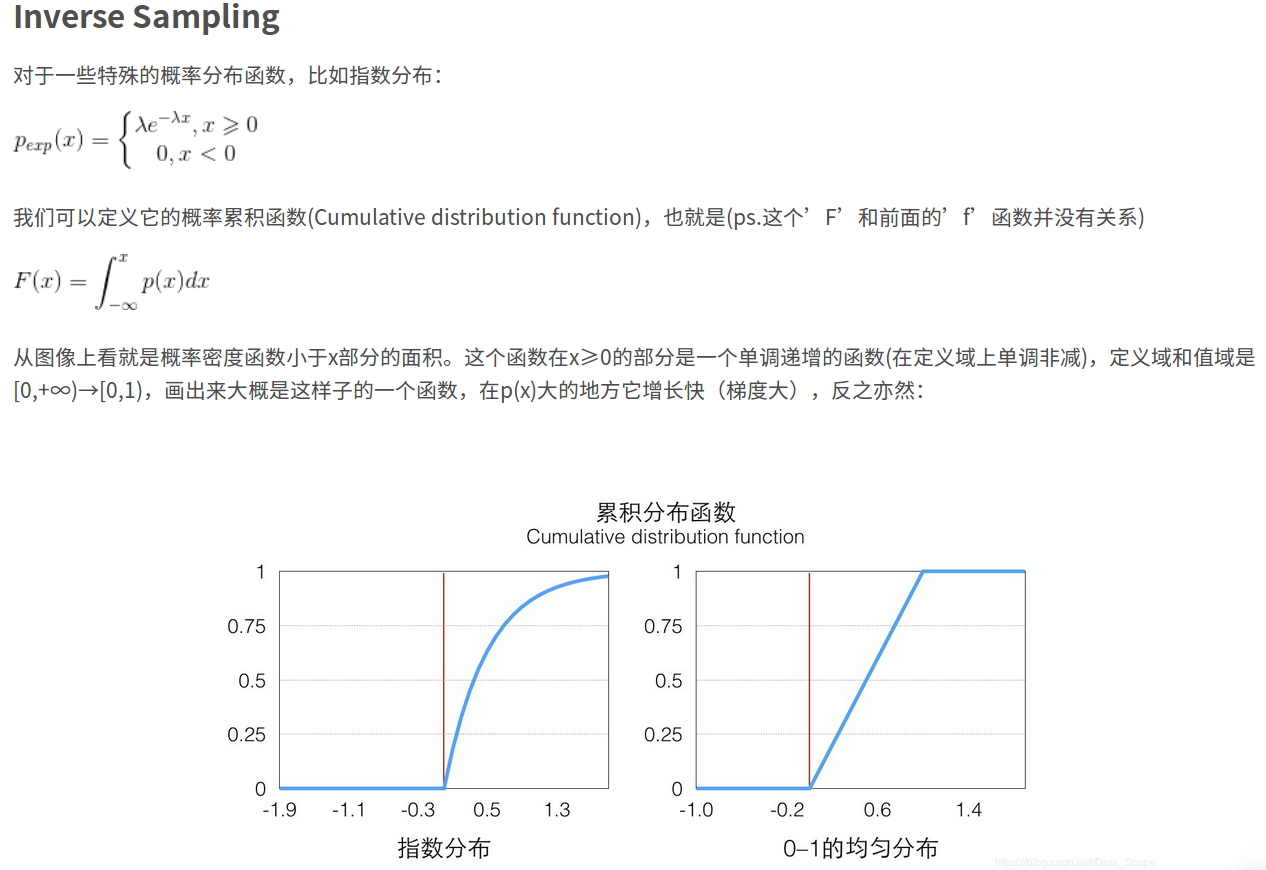
\includegraphics[scale=0.4]{15.png}}
				\end{figure}
				\begin{figure}[H]
					\centering{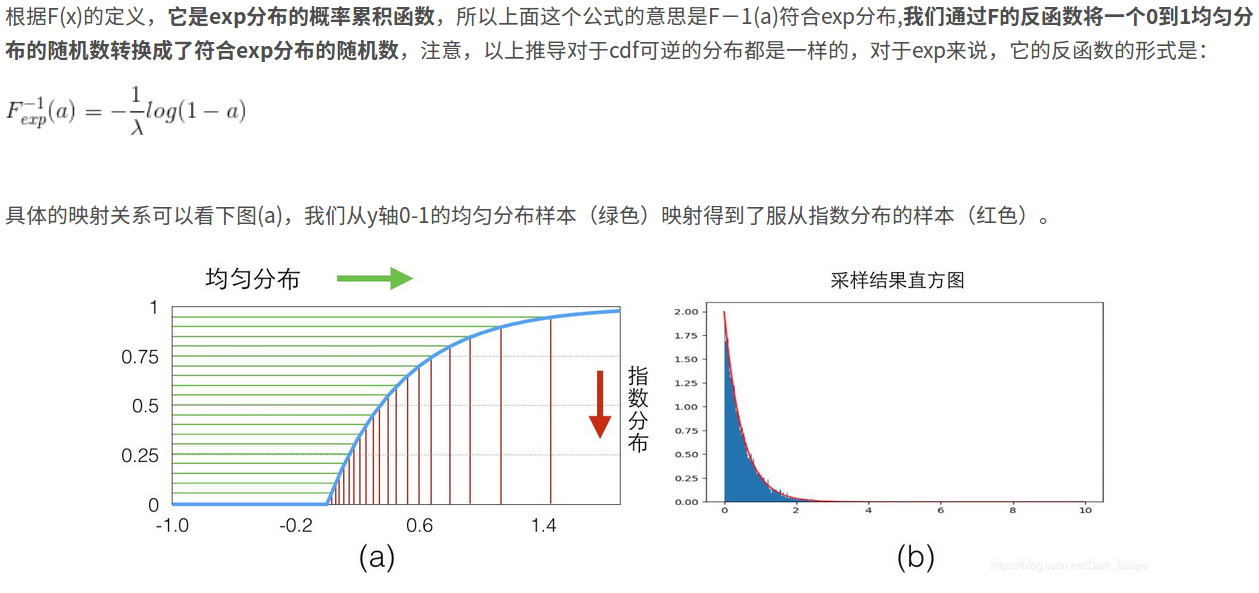
\includegraphics[scale=0.4]{16.png}}
				\end{figure}
			\subsection{拒绝采样}
				\begin{figure}[H]
					\centering{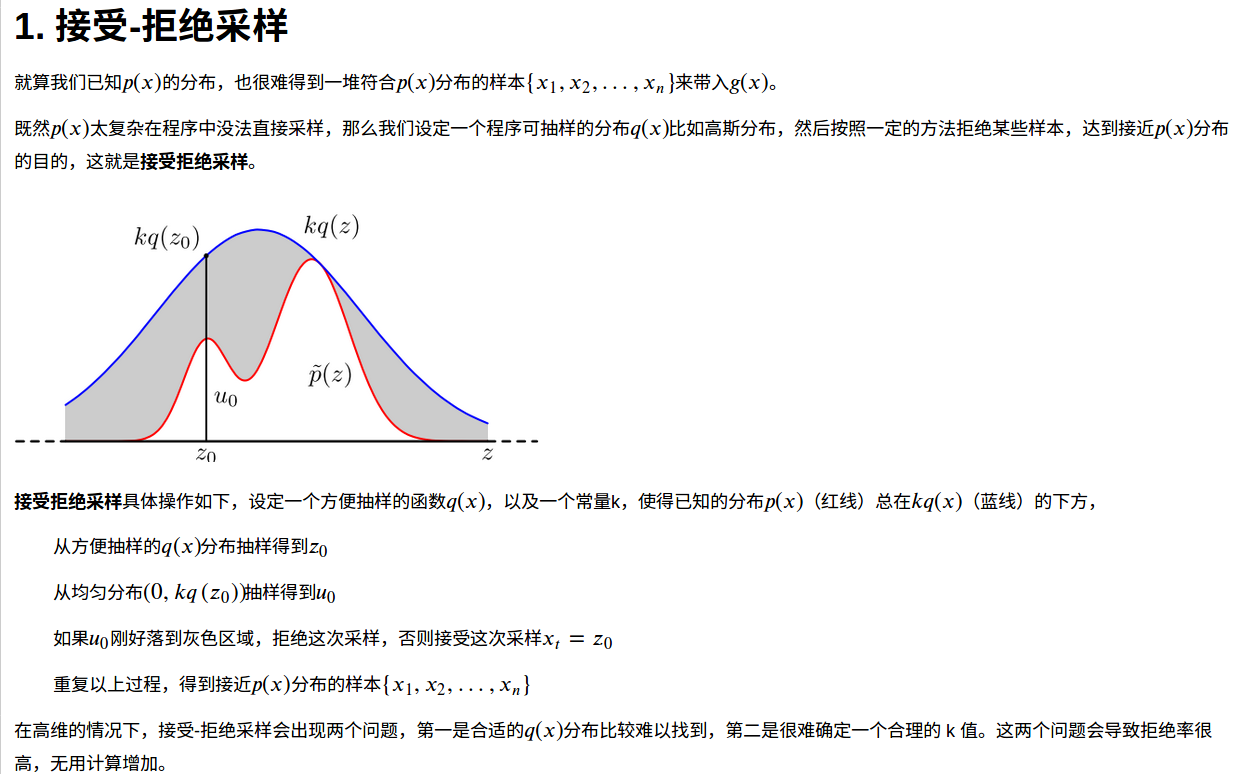
\includegraphics[scale=0.4]{10.png}}
				\end{figure}
				\begin{figure}[H]
					\centering{
\includegraphics[scale=0.4]{11.png}}
				\end{figure}
				\begin{figure}[H]
					\centering{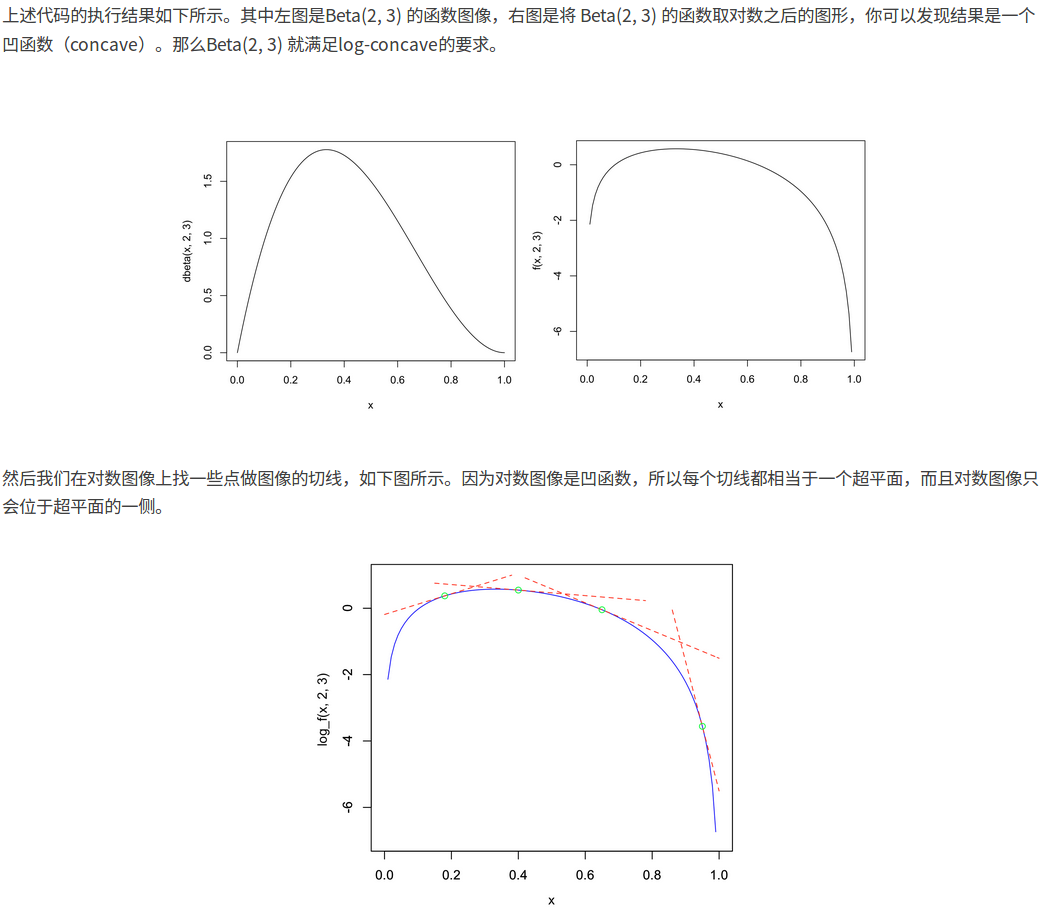
\includegraphics[scale=0.4]{12.png}}
				\end{figure}
				\begin{figure}[H]
					\centering{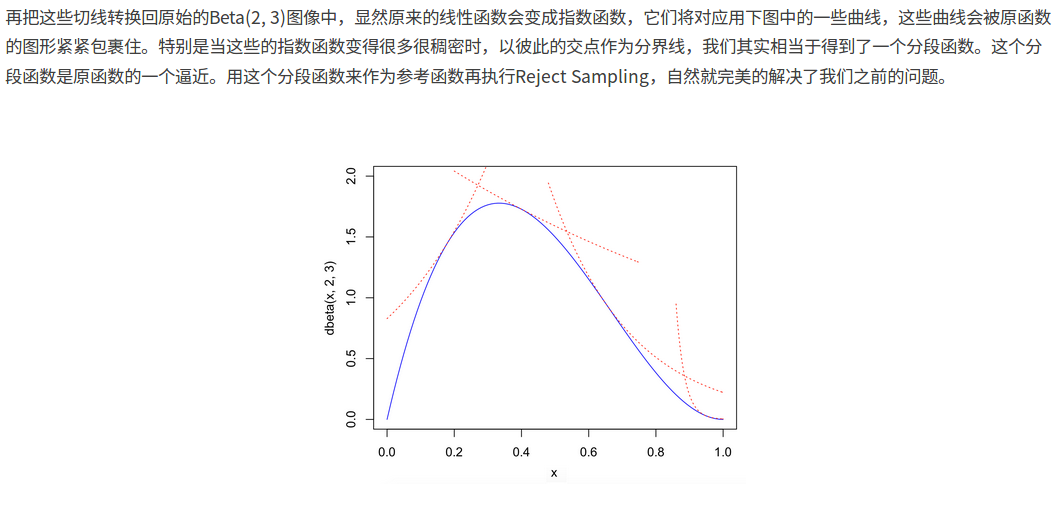
\includegraphics[scale=0.4]{13.png}}
				\end{figure}	
			\subsection{重要性采样}
				\begin{figure}[H]
					\centering{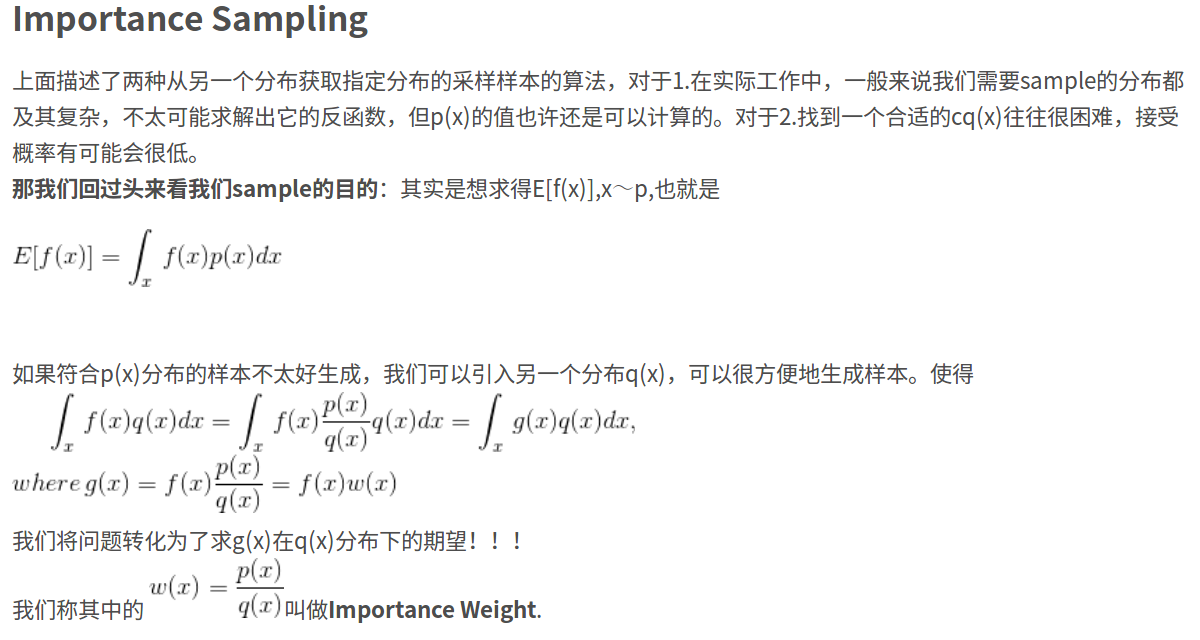
\includegraphics[scale=0.4]{14.png}}
				\end{figure}
				在高维情况下,上面的方法都不太行。
			\subsection{马尔科夫链的平稳分布}
				在马尔科夫链中,如果其状态空间为$\{1,2,\cdots,k\}$,条件转移矩阵(随机矩阵,特征值的绝对值小于等于1):
				\[\begin{pmatrix}
				Q_{11}&Q_{12}&\cdots&Q_{1k}\\
				Q_{21}&Q_{22}&\cdots&Q_{2k}\\
				\vdots&\vdots&\vdots&\vdots\\
				Q_{k1}&Q_{k2}&\cdots&Q_{kk}\\
				\end{pmatrix}\]
				
				则第t+1个时刻,样本x=j的概率:
				\[q^{(t+1)}(x=j) = \sum_{i=1}^kq^{(t)}(x=i)Q_{ij}\]
				
				把第t+1个时刻样本所有取值的概率写成一个向量:
				\[\bm{q^{(t+1)}} = \Big(q^{(t+1)}(x=1)\quad q^{(t+1)}(x=2)\cdots q^{(t+1)}(x=k)\Big)\]
				代入可得:
				\[\begin{aligned}
				\bm{q^{(t+1)}} &= \Bigg(\underbrace{\sum_{i=1}^kq^{(t)}(x=i)Q_{i1}}_{\text{每一列和}}\quad \sum_{i=1}^kq^{(t)}(x=i)Q_{i2}\cdots \sum_{i=1}^kq^{(t)}(x=i)Q_{ik}\Bigg)\\
				&=\bm{q^{(t)}}\bm{Q}
				\end{aligned}\]
				所以:
				\[\bm{q^{(t+1)}} = \bm{q^{(t)}}\bm{Q}=\cdots=\bm{q^{(1)}}\bm{Q}^t \]
				将随机矩阵特征值分解,不妨设$\lambda_i=1$:
				\[\bm{Q} = \bm{A\Lambda A}^{-1}\]
				所以,经过足够多的m次采样(收敛的时间叫做mixing time):
				\[\bm{q^{(t+1)}} = \bm{q^{(1)}}\bm{A\Lambda^m A}^{-1}\]
				\[s.t.\quad\bm{\Lambda}^m = \begin{pmatrix}
				0& & & & \\
				&\ddots\\
				&&1\\
				&&&\ddots\\
				&&&&0\\
				\end{pmatrix}\]
				当t>m时,后面的分布都相同了:
				\[\bm{q^{(m+1)}} = \bm{q^{(m+2)}}=\cdots=\bm{q^{(\infty)}}\]
				
				存在问题:理论上只能保证收敛性无法知道何时收敛;混合时间过长(高维,维度之间相关性强);样本之间有一定的相关性。当分布是多峰的时候,样本很容易就只在一个峰里面打转,很难突破最低值到达另一个峰,造成混合时间太长。
				\begin{figure}[H]
					\centering{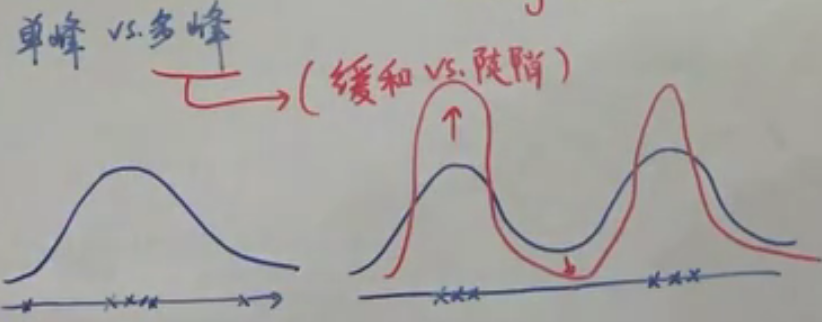
\includegraphics[scale=0.4]{21.png}}
				\end{figure}
			
			
			
			
			\subsection{MCMC}
				马尔科夫链的时间和状态都是离散的,P是状态转移矩阵。
				\[\pi(x^*) = \int \pi(x)P(x\rightarrow x^*)dx\]
				如果分布${\pi(k)}$满足上式,则称${\pi(k)}$为${X_t}$的\uline{平稳分布}。
				
				满足\uline{细致平衡}条件,则可推出$\pi$为平稳分布(两个点之间能跳过来也能跳过去):
				\[\pi(x)P(x\rightarrow x^*) = \pi(x^*)P(x^*\rightarrow x)\]
				\textbf{Metropolis Hasting:}
				\begin{figure}[H]
					\centering{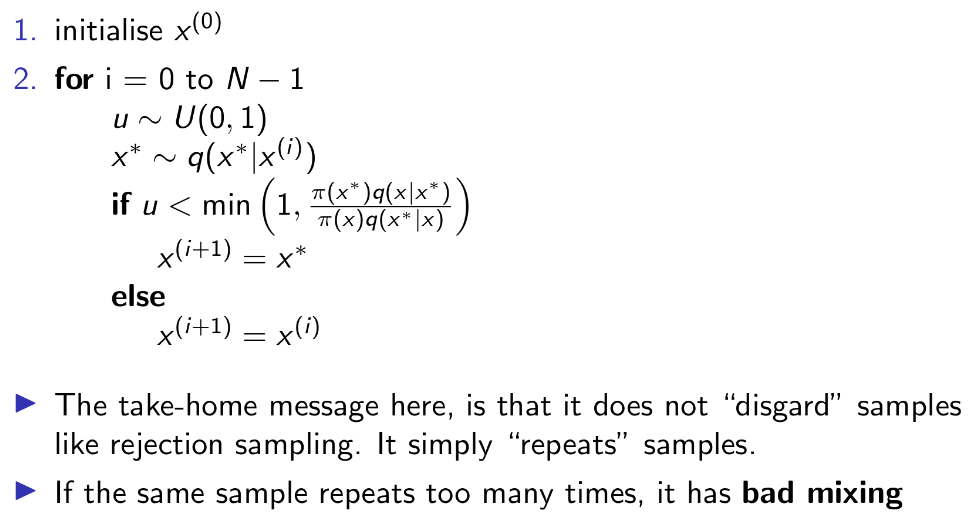
\includegraphics[scale=0.4]{17.png}}
				\end{figure}	
				\begin{figure}[H]
					\centering{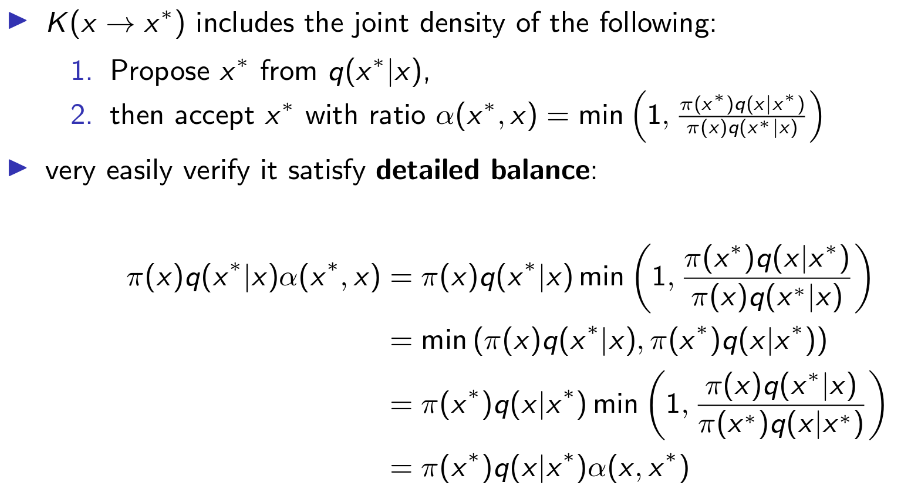
\includegraphics[scale=0.4]{18.png}}
				\end{figure}		
				\textbf{吉布斯采样:}	
				\begin{figure}[H]
					\centering{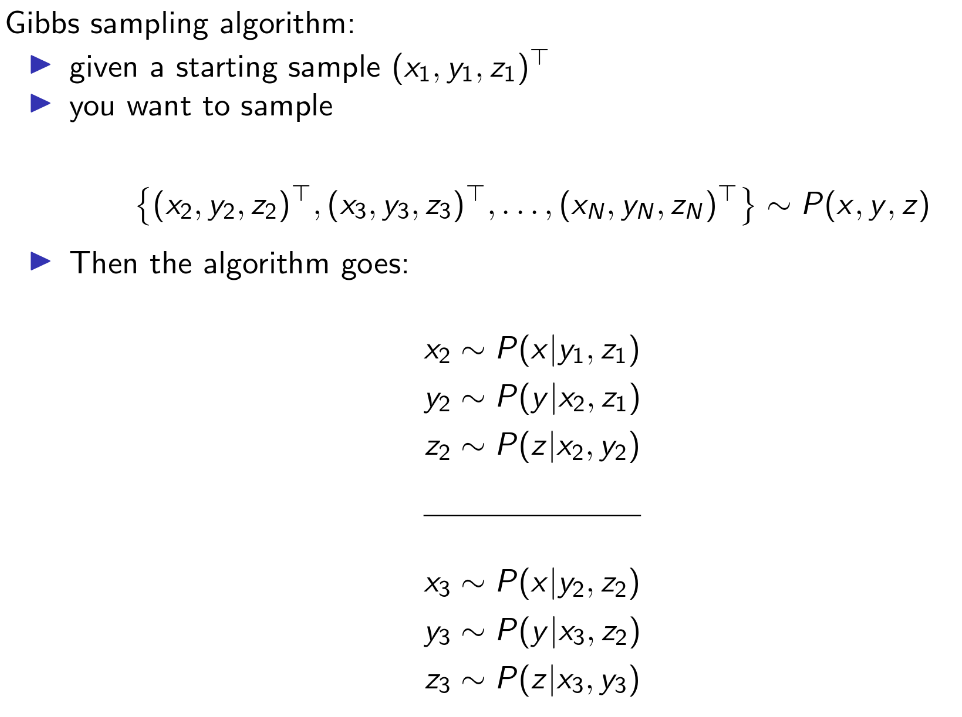
\includegraphics[scale=0.4]{19.png}}
				\end{figure}	
				吉布斯采样其实是MH采样的接受率为1的一种特殊情况。
				\begin{figure}[H]
					\centering{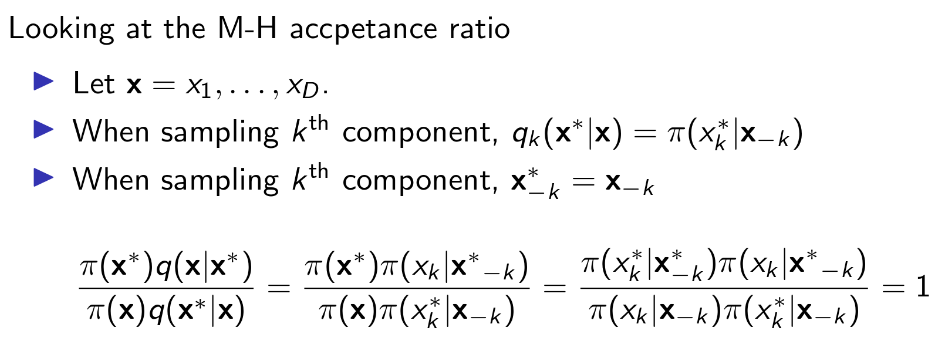
\includegraphics[scale=0.4]{20.png}}
				\end{figure}
				下标$X_{-k}$表示X的除去k的所以维度。
				
				吉布斯采样就是把目标分布P对应的条件概率当做状态转移分布Q。\\
				
				\textbf{采样的动机:}
				
				\quad1.采样本身就是常见的额任务
				
				\quad12.求和或求积分
				
				\textbf{什么是好的样本?}
				
				\quad11.样本趋向于高概率区域
				
				\quad1 2.样本之间相互独立
				
				\textbf{采样困难:(高维)}
				
				\quad1.归一化系数无法求解
				
				\quad2.维度太高,无法直接采样(需知道每个状态的概率,要遍历)\\
				
				拒绝采样与重要性采样都构造了一个分布q,1.要求q与p接近,2.且q要更简单。
			
		
			
			
			
			
\end{document}